<<<<<<< HEAD
%%%%%%%%%%%%%%%%%%%%%%%%%%%%%%%%%%%%%%%%%%%
%%%%%%  STYLE 33
%%%%%%%%%%%%%%%%%%%%%%%%%%%%%%%%%%%%%%%%%%%
\restoregeometry
\cxset{style33/.style={
 name=CHAPTER,
 numbering=arabic,
 number font-size=\LARGE,
 number font-family=\rmfamily,
 number font-weight=\normalfont,
 number before={\par\hfill},
 number after={\hfill\hfill\par},
 number position=leftname,
 name=,
 chapter font-family=\sffamily,
 chapter font-weight=\normalfont,
 chapter font-size=\small,
 chapter before={\vskip10pt},
 chapter after={\vskip10pt\par},
 chapter color={black!90},
 number color=\color{black!90},
 title beforeskip={},
 title afterskip={\vspace{50pt}},
 title before=\hfill,
 title after={\hfill\hfill\par},
 title font-family=\normalfont,
 title font-color=\color{black!80},
 title font-weight=\normalfont,
 title font-shape=\upshape,
 title font-size=\LARGE,
 section numbering=none,
 section font-size=\Large,
 section align=\centering}}

\cxset{style33}
\chapter{Introduction to Style Thirty Three}

The interesting part of this style is that it uses roman numerals to display the counter that is in a different font than that used for the chapter name.
\medskip
\begin{figure}[ht]
\centering
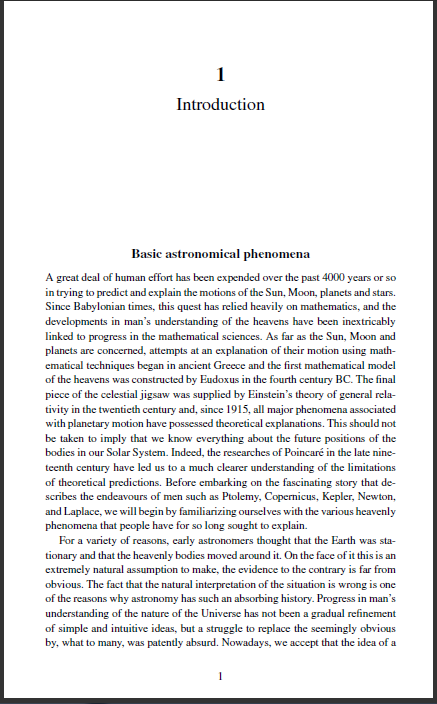
\includegraphics[width=0.6\textwidth]{./chapters/chapter33}
\end{figure}

=======
%%%%%%%%%%%%%%%%%%%%%%%%%%%%%%%%%%%%%%%%%%%
%%%%%%  STYLE 33
%%%%%%%%%%%%%%%%%%%%%%%%%%%%%%%%%%%%%%%%%%%
\restoregeometry
\cxset{style33/.style={
 name=CHAPTER,
 numbering=arabic,
 number font-size=\LARGE,
 number font-family=\rmfamily,
 number font-weight=\normalfont,
 number before={\par\hfill},
 number after={\hfill\hfill\par},
 number position=leftname,
 name=,
 chapter font-family=\sffamily,
 chapter font-weight=\normalfont,
 chapter font-size=\small,
 chapter before={\vskip10pt},
 chapter after={\vskip10pt\par},
 chapter color={black!90},
 number color=\color{black!90},
 title beforeskip={},
 title afterskip={\vspace{50pt}},
 title before=\hfill,
 title after={\hfill\hfill\par},
 title font-family=\normalfont,
 title font-color=\color{black!80},
 title font-weight=\normalfont,
 title font-shape=\upshape,
 title font-size=\LARGE,
 section numbering=none,
 section font-size=\Large,
 section align=\centering}}

\cxset{style33}
\chapter{Introduction to Style Thirty Three}

The interesting part of this style is that it uses roman numerals to display the counter that is in a different font than that used for the chapter name.
\medskip
\begin{figure}[ht]
\centering
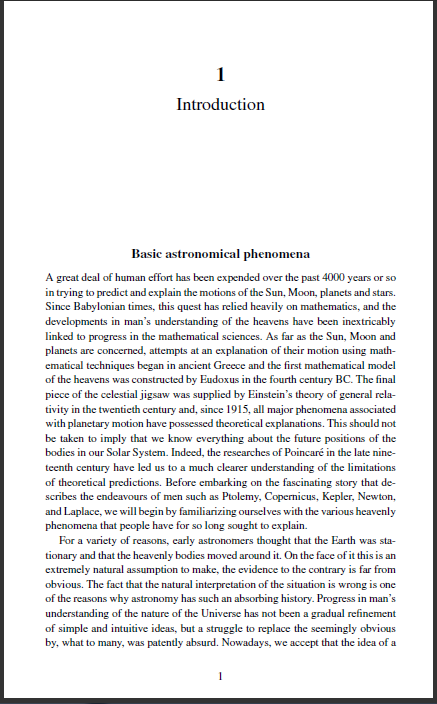
\includegraphics[width=0.6\textwidth]{./chapters/chapter33}
\end{figure}

>>>>>>> merged
